\documentclass{article}

\usepackage{tikz-qtree}
\usepackage{tikz}

\author{Yeoun Chan Kim \and John Strauser \and Xuanang Wang}

\title{CS440 Assignment2}

\begin{document}

\maketitle

\section*{P1}

\hspace{5mm}

Expansion sequence:

Start

(Lugoj, f=244, g=0, h=244)

Expand Lugoj:

(Mehadia, f=311, g=70, h=241)

(Timisoara, f=440, g=111, h=329)

Expand Mehadia

(Drobeta, f=387, g=145, h=242)

Expand Drobeta

(Craiova, f=425, g=265, h=160)

Expand Craiova

(Pitesti, f=503, g=403, h=100)

(Rimnicu Vilcea, f=604, g=411, h=193)

Expand Timisoara (440 < 503 < 604)

(Arad, f=565, g=229, h=336)

Expand Pitesti (503 < 565 < 604)

(Bucharest, f=504, g=504, h=0) 

We can stop here because f(Bucharest) $<$ f(Arad) $<$ f(Rimnicu Vilcea)

\section*{P2}

\hspace{5mm}

A)

BFS:

State 1 expands to State 2 and 3

State 2 expands to State 4 and 5

State 3 expands to State 6 and 7

State 4 expands to State 8 and 9

State 5 expands to State 10 and 11

State 6 expands to State 12 and 13

State 7 expands to State 14 and 15

State 8 expands to State 16 and 17

State 9 expands to State 18 and 19

State 10 expands to State 20 and 21

State 11 is found and the search stops

\hspace{5mm}

Depth-Limited:

State 1 expands to State 2 and 3

State 2 expands to state 4 and 5

State 4 expands to state 8 and 9

State 8 expands to state 16 and 17

Wont expand 16 and 17 due to depth limit of 3

State 9 expands to state 18 and 19

Wont expand 18 and 19 due to depth limit of 3

State 5 expands to state 10 and 11

State 10 expands to state 20 and 21

Wont expand 20 and 21 due to depth limit of 3

State 11 is found and the search stops

\hspace{5mm}

Iterative Deepening:

limit starts at 0

State 1 expands to state 2 and 3
\newline

limit is increased to 1

State 1 expands to state 2 and 3

State 2 expands to State 4 and 5

State 3 expands to State 6 and 7
\newline

limit is increased to 2

State 1 expands to state 2 and 3

State 2 expands to State 4 and 5

State 4 expands to State 8 and 9

State 5 expands to State 10 and 11

State 3 expands to State 6 and 7

State 6 expands to State 12 and 13

State 7 expands to State 14 and 15
\newline

limit is increased to 3

State 1 expands to state 2 and 3

State 2 expands to State 4 and 5

State 4 expands to State 8 and 9

State 8 expands to State 16 and 17

State 9 expands to State 18 and 19

State 5 expands to State 10 and 11

State 10 expands to State 20 and 21

State 11 is found and the search stops

\hspace{5mm}

B)

Bidirectional sort should be optimal for this problem since all edges have the same undefined cost.
\newline

Order:

State 1 expands to state 2 and 3

State 11 expands to state 5

State 2 expands to state 4 and 5

State 5 expands to state 2, which has already been expanded so the search is complete
\newline


Branching factor for the downward search (starting at state 1) is 2.

Branching factor for the upward search (starting at state 11) is 1.

\section*{P3}

\hspace{5mm}

a) True

b) True

c) True

d) False

e) True

f) True

g) True

h) False

i) True

\section*{P4}

\hspace{5mm}

Advantage: Iterative Deepening requires less memory overall compared to BFS.

Disadvantage: Becuase Iterative Deepening restarts the search each time the depth-limit is increased, the amount of nodes expanded is significantly higher.

\section*{P8}

\hspace{5mm} 

1) A heuristic function h is said to be admissible if for any state n, the heuristic value of the state h{\small (n)} is less or equal to the heuristic value of the goal state h{\small (g)}.

a) Given the fact that both h{\small 1(n)} and h{\small 2(n)} are admissible, h{\small (n)} would be admissible because either h{\small 1(n)} or h{\small 2(n)} overestimate the cost to reach the h{\small (g)}. In this case, the smaller one of those two would still obtain a cost which smaller or equal to the real cost to reach the h{\small (g)} therefore admissible.

b) We consider the given function at the boundary position:
\begin{center}

when w = 0, h{\small(n)} = h{\small 2(n)}

when w = 1, h{\small(n)} = h{\small 1(n)}

\end{center}

Because of the fact that both h{\small 1(n)} and h{\small 2(n)} are admissible, we can see h{\small(n)} remains admissible for both boundaries.

Furthermore, we want to prove that the given function remains admissible for any value within the interval 0 $<$ w $<$ 1. Again, because of the fact that both h{\small 1(n)} and h{\small 2(n)} are admissible, no matter which value in the interval is chosen,  h{\small (n)} would always obtain a value which smaller than either h{\small 1(n)} or h{\small 2(n)} which would not exceed the cost to reach h{\small (g)} therefore is admissible.

c) Given the fact that both h{\small 1(n)} and h{\small 2(n)} are admissible, h{\small (n)} would be admissible because either h{\small 1(n)} or h{\small 2(n)} overestimate the cost to reach the h{\small (g)}. In this case, even if we want to choose the larger one, it would still obtain a cost which smaller or equal to the real cost to reach the h{\small (g)} therefore admissible.

\vspace{5mm}

2) A heuristic function h is said to be consistent if for any state n, the heuristic value of the state h{\small(n)} is less or equal than the cost c{\small(n')} to go to state n' starting from n plus the heuristic value of that state h{\small(n')}

\begin{center}

h{\small(n)} $\le$ c{\small(n')} + h{\small(n')}

\end{center}

There are plenty of explanations being done in part 1), therefore we are going to explain 2) in a simple way. Through observation in part 1), we can notice that none of three functions would return a value which make h{\small(n)} larger than either of h{\small1(n)} or h{\small2(n)}. Therefore, given the fact that both h{\small 1(n)} and h{\small 2(n)} satisfies the equation above, a value smaller or equal to h{\small 1(n)} or h{\small 2(n)} would still satisfies the equation above; therefore remain consistent.

\section*{P9}

\hspace{5mm} 

a) Hill climbing works better than simulated annealing when the objective function has only one global maximum and without plateaux.

b) The hill-climbing part of simulated annealing is not necessary when the maximum (peek) value in the objective function is relatively or completely flat.

c) Simulated annealing is useful when the local/global maximum of objective function is relatively sharp, the objective function has a lot local maximum with plateaux or shoulder situation.

d) The simulated annealing would return a value which is or near the global maximum. Because of the fact that it does not often return the best solution, given that we know the value (measure of goodness) of each state we visit, we can compare the current state with it's neighbors and return the one which has the best measure of goodness.

e) Since the formal simulated annealing only stores the current and the next state, there would be a lot redundancy work being done when running the algorithm. However, given that we have enough memory to hold more information, we can simply start from the beginning of the objective function, traverse and store each state's measure of goodness until the end of the objective function. Then, we just pick the one which has the best measurement of goodness as return value.

f) The key of gradient ascent search is calculate the gradient of the objective function at current state and take step proportional to the gradient if it is positive. If the current state is at local maximum, all of it's neighbor would have a negative gradient therefore the agent would stuck. Because of the fact that the method of hill climbing is similar to gradient ascent search, we may just replace the role that is done by hill climbing in simulated annealing using gradient ascent search in order to avoid being stuck.

\section*{P10}

For the following tree, each state have a format of K(P1, P2)(C) where K represents which player's move, P1 represents the current token position for player A, P2 represents the current token position for player B, C represents the minmax value of the state. Note: the end state has no K.

\tikzset{every tree node/.style={minimum width=2em,draw,blank},
         blank/.style={draw=none},
         edge from parent/.style=
         {draw,edge from parent path={(\tikzparentnode) -- (\tikzchildnode)}},
         level distance=1.5cm}
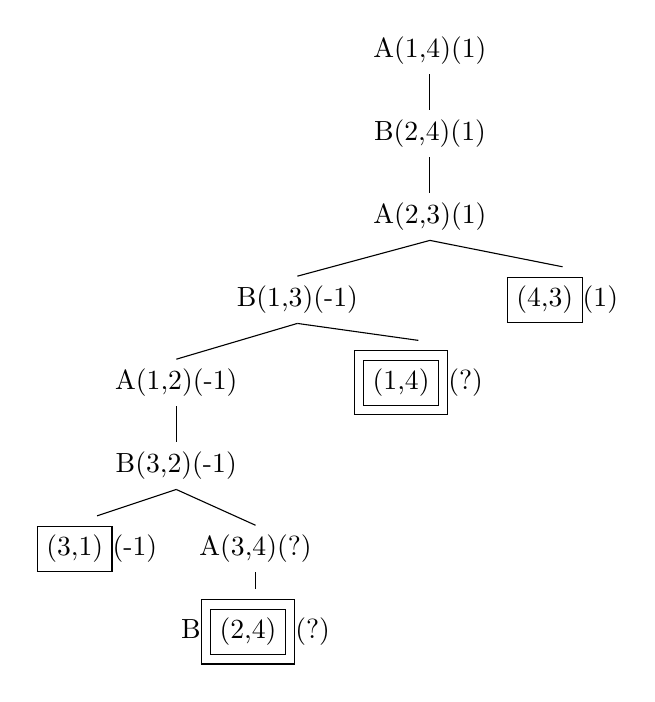
\begin{tikzpicture}
\Tree
[.A(1,4)(1)
%\edge[blank]; \node[blank]{};
\edge[];
    [.B(2,4)(1)
   %\edge[blank]; \node[blank]{};
    \edge[];
        [.A(2,3)(1)
        \edge[];
            [.B(1,3)(-1)
                \edge[];
                [.A(1,2)(-1)
                \edge[];
                    [.B(3,2)\\(-1)
                    \edge[];
                        [.\framebox{(3,1)}\\(-1)
                           % \edge[blank];{-1}
                        ]
                    \edge[];
                        [.A(3,4)\\(?)
                        \edge[];{B\framebox{\framebox{(2,4)}}}\\(?)
                        ]
                    ]
                ]
                \edge[];
                    [.\framebox{\framebox{(1,4)}}\\(?)
                    ]
            ]
            \edge[];
                [.\framebox{(4,3)}\\(1)
                    %\edge[blank];{1}
                ]
        ]
    %\edge[blank]; \node[blank]{};
    ]
%\edge[blank]; \node[blank]{};
]
\end{tikzpicture}

\vspace{5mm}
\hspace{5mm}
We assume that both player wants to maximize his/her value while minimizing his/her opponent's. Therefore, as player A's perspective, the game would be ended at the line 4 therefore there is no need to worry about the "?" values.

\end{document}
